\documentclass[xcolor={dvipsnames}]{beamer}
\usepackage{color, colortbl}
\usepackage[ngerman,english]{babel}
\usepackage[T1]{fontenc}
%\usepackage{CJKutf8} %japanese
\usepackage{lmodern}
\usepackage[compatibility=false]{caption}
\usepackage{subcaption}
\usepackage{tikz}
\usepackage{textgreek}
\usepackage{tabularx}
\usepackage{booktabs}
\usepackage{siunitx}
\usepackage{appendixnumberbeamer}
\usepackage[absolute,overlay]{textpos} %for positioning the logos where I want
\usepackage{xspace,multicol}

\usepackage{animate}
\usepackage{multimedia}

\mode<presentation>
{
  \usetheme{CambridgeUS}     
  \usecolortheme{lily} 
  \definecolor{beamer@violet}{rgb}{0.5,0.3,0.5} % changed this
  \setbeamercolor{structure}{fg=beamer@violet!70!cyan}
  \setbeamercolor{palette primary}{fg=black, bg=gray!30!white!50!cyan!20!}
  \setbeamercolor{palette secondary}{fg=black, bg=gray!30!white!30!cyan!40!}
  \setbeamercolor*{palette tertiary}{bg=gray!20!white!20!cyan!60!}
  
  \setbeamercolor{frametitle}{fg=cyan!60!white!40!,bg=cyan!80!black}
  \setbeamercolor{title}{fg=cyan!80!black}
  \setbeamercolor{normal text}{fg=black,bg=white}
  \setbeamercolor{alerted text}{fg=beamer@violet}
  \setbeamercolor{example text}{fg=beamer@violet!70!cyan}
  
  \usefonttheme{structureitalicserif} 
  \setbeamertemplate{navigation symbols}{}
  \setbeamertemplate{caption}[numbered]
}
\newcommand{\sidlogo}{
  \setlength{\TPHorizModule}{1pt}
  \setlength{\TPVertModule}{1pt}
   % textblock{}{x,y}: pos(x) = rightUpperCorner + (x * \TPHorizModule), pos(y) = leftUpperCorner - (y * \TPVertModule)
  \begin{textblock}{1}(323,12)
   \includegraphics[width=40pt,height=26pt]{figures/SiD.jpeg}
  \end{textblock}
  } 
\newcommand{\ilclogo}{
  \setlength{\TPHorizModule}{1pt}
  \setlength{\TPVertModule}{1pt}
   % textblock{}{x,y}: pos(x) = rightUpperCorner + (x * \TPHorizModule), pos(y) = leftUpperCorner - (y * \TPVertModule)
  \begin{textblock}{1}(323,12)
   \includegraphics[width=40pt,height=26pt]{figures/ILC.jpeg}
  \end{textblock}
} 
\newcommand{\flukalogo}{
  \setlength{\TPHorizModule}{1pt}
  \setlength{\TPVertModule}{1pt}
   % textblock{}{x,y}: pos(x) = rightUpperCorner + (x * \TPHorizModule), pos(y) = leftUpperCorner - (y * \TPVertModule)
  \begin{textblock}{1}(315,12)
   \includegraphics[width=60pt,height=26pt]{figures/fluka_logo.png}
  \end{textblock}
} 
\newcommand{\ejadelogo}{
  \setlength{\TPHorizModule}{1pt}
  \setlength{\TPVertModule}{1pt}
   % textblock{}{x,y}: pos(x) = rightUpperCorner + (x * \TPHorizModule), pos(y) = leftUpperCorner - (y * \TPVertModule)
  \begin{textblock}{1}(323,12)
   \includegraphics[width=40pt,height=26pt]{figures/EJADE.jpeg}
  \end{textblock}
} 
\newcommand{\BDSsymbol}{
  \setlength{\TPHorizModule}{1pt}
  \setlength{\TPVertModule}{1pt}
   % textblock{}{x,y}: pos(x) = rightUpperCorner + (x * \TPHorizModule), pos(y) = leftUpperCorner - (y * \TPVertModule)
  \begin{textblock}{1}(0,39)
   \includegraphics[width=60pt,height=40pt]{figures/Highlight_BDS.png}
  \end{textblock}
} 
\newcommand{\EXTsymbol}{
  \setlength{\TPHorizModule}{1pt}
  \setlength{\TPVertModule}{1pt}
   % textblock{}{x,y}: pos(x) = rightUpperCorner + (x * \TPHorizModule), pos(y) = leftUpperCorner - (y * \TPVertModule)
  \begin{textblock}{1}(0,39)
   \includegraphics[width=60pt,height=40pt]{figures/Highlight_EXT.png}
  \end{textblock}
} 
\newcommand{\ATFlogo}{
  \setlength{\TPHorizModule}{1pt}
  \setlength{\TPVertModule}{1pt}
   % textblock{}{x,y}: pos(x) = rightUpperCorner + (x * \TPHorizModule), pos(y) = leftUpperCorner - (y * \TPVertModule)
  \begin{textblock}{1}(323,12)
   \includegraphics[width=40pt,height=26pt]{figures/ATF_logo.jpg}
  \end{textblock}
} 
\newcommand{\rhullogo}{
  \setlength{\TPHorizModule}{1pt}
  \setlength{\TPVertModule}{1pt}
   % textblock{}{x,y}: pos(x) = rightUpperCorner + (x * \TPHorizModule), pos(y) = leftUpperCorner - (y * \TPVertModule)
  \begin{textblock}{1}(343,12)
   \includegraphics[width=20pt,height=26pt]{figures/rhul_logo.png}
  \end{textblock}
}

\DeclareSIUnit\year{yr}
\newcommand{\eplus}{e$^+$\xspace}
\newcommand{\eminus}{e$^-$\xspace}

\title[ATF2 Background Simulations]{\textbf{Vertical Collimator System\\for Background Suppression at ATF2\\\small{Data Analysis and BDSIM Simulation}}}
\author{\textbf{Anne Sch\"utz}}
\institute{\textbf{KIT, DESY}}
\date{\textbf{\today}}

\titlegraphic{\includegraphics[height=1.0cm]{figures/KIT.png}\hspace*{6cm}~%
   \includegraphics[height=1.2cm]{figures/DESY_Logo.png}
}

\begin{document}

{
\usebackgroundtemplate{
 \tikz\node[opacity=0.1]{\includegraphics[width=\paperwidth]{figures/Iwatecomics.jpg}};
 % \tikz\node[opacity=0.2]{\centering\includegraphics[height=\paperheight]{figures/Iwatecomics.jpg}};
 }
\begin{frame}
  \titlepage
\end{frame}
}

%\begin{frame}{Table of contents}
%  \tableofcontents
%\end{frame}

%--------------------------------------------------------------

\section{Ongoing projects around background simulations}
\begin{frame}{My Ph.D topic}
 \begin{block}{}
  \centering
  \textit{Optimizing the design of the Final-Focus Region\\for the International Linear Collider}
  \end{block}
  \vspace*{0.5cm}
  I study different background sources occurring in the interaction region of the ILC to find limits and requirements of the FF region design.
\end{frame}

\subsection{Background simulations}

\begin{frame}{Background sources}
\ilclogo
The main sources of background:
\begin{columns}
 \begin{column}{0.55\textwidth}
  \begin{itemize}
    \item Pair background
    \item Bhabha scattering
    \item \textgamma \textgamma $\rightarrow$ hadrons
    \item \emph{Neutrons from the beam dumps}
    \item Background from Final-Focus system (\emph{beam halo collimators}, muon spoilers)
  \end{itemize}
 \end{column}
 \begin{column}{0.45\textwidth}
 \includegraphics[height=0.2\textheight]{figures/beamstrahlung_processes.png}\\
 \includegraphics[height=0.15\textheight]{figures/bhabha_scattering.pdf} 
 \includegraphics[height=0.15\textheight]{figures/gammagamma_hadrons.pdf}
 \end{column}
\end{columns}

\end{frame}




\section{The Final-Focus system as a background source}
\begin{frame}
\ATFlogo
 \begin{center}
    \LARGE ATF2 background study for the\\vertical beam halo collimator
 \end{center}
\end{frame}

\begin{frame}{Vertical Beam Halo collimators}
Vertical collimators suggested for the ILC:\\
 \begin{center}
\includegraphics[width=0.65\textwidth]{figures/ATF2_beamhalo_collimator.pdf}
\end{center}
In the ATF2 beam operation weeks between March and October 2016:
\begin{itemize}
\item Installing the new vertical beam halo collimator
\item Measuring the beam halo, the background and the wake fields
\item Studies of the generated background in the proximity of the collimator with the RHUL Cherenkov detector
\end{itemize}

\end{frame}

\begin{frame}{Installed collimator}
\ATFlogo

\begin{center}
\includegraphics[width=\textwidth]{figures/ATF2schematic.pdf}\\
 \includegraphics[width=0.5\textwidth]{figures/Installed_Collimator.jpg}
\end{center}
\end{frame}

\begin{frame}{Data analysis}
\ATFlogo
Data taken with the RHUL Cherenkov detector\\
\vspace*{0.4cm}
 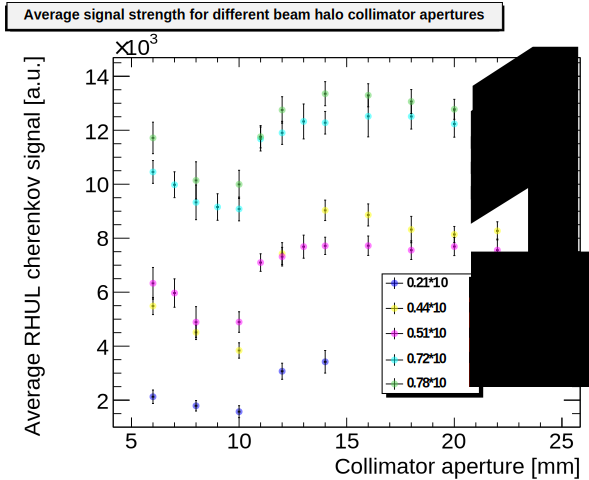
\includegraphics[height=0.55\textheight]{figures/AverageSignal_perAperture.png}
  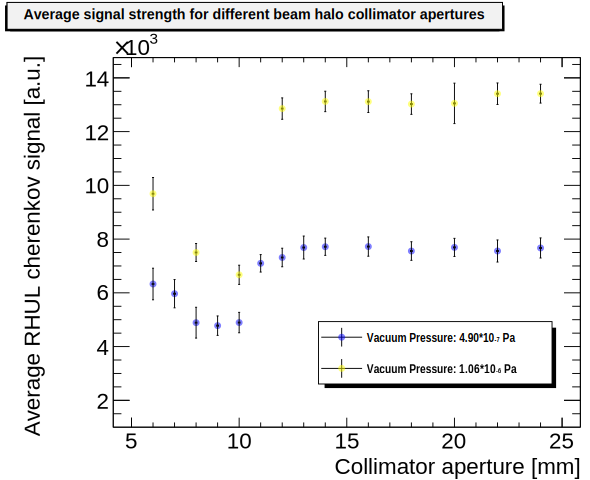
\includegraphics[height=0.55\textheight]{figures/AverageSignal_perAperture_VacuumPressures.png}\\
The background is reduced, but then rises again when collimator jaws are driven closer into the beam halo.\\
\small The vertical beam size at the location of the collimator was about \SI{0.32}{mm} with an offset of 0.2-\SI{0.5}{mm}.
\end{frame}

\begin{frame}{Data analysis}
\ATFlogo
Data taken with the post-IP background monitor\\
\vspace*{0.3cm}
\begin{center}
  \includegraphics[width=0.8\textwidth]{figures/Nuria_postIP_Bkg_VerticalCollimator.png}\\
\end{center}
Preliminary results by Nuria Fuster Martinez (IFIC, Spain)\\
\Large{$\Rightarrow$ Background is reduced at the IP.}
\end{frame}

\begin{frame}{Plans for the BDSIM simulation}
\rhullogo
Plans for the BDSIM study:
\begin{itemize}
 \item Comparing the data taken at ATF with the simulation results.
 \item Understanding where background particles are generated and stopped exactly.
\end{itemize}

\begin{center}
  \includegraphics[width=0.8\textwidth]{figures/atf_bdsim.png}\\
\end{center}

Data taken:
\begin{columns}
 \begin{column}[c]{0.6\textwidth}
\begin{itemize}
 \item Scans of the collimator aperture (symmetrically, and jaws individually)
 \item Scans with the fixed aperture
 \item At different beam intensities
 \item At different vacuum pressures
\end{itemize}
 \end{column}
  \begin{column}[c]{0.4\textwidth}
 \centering

\includegraphics[width=\textwidth]{figures/Jaw_movements.png}\\
 \end{column}
 \end{columns}

\end{frame}

\begin{frame}
What is needed from the BDSIM simulation:
\begin{itemize}
 \item Setting the collimator aperture
 \item Individual movement of the collimator jaws
 \item Setting the position of the collimator {\small{(synchronous jaw movement when aperture is fixed)}}
 \item Changing the vacuum pressure in the model
 \item Changing the beam orbit offset
 \item Finding the particle vertexes
\end{itemize}


\begin{columns}
\begin{column}[c]{0.2\textwidth}
 \centering
\includegraphics[height=0.5\textheight]{figures/ROOT_Tree1.png}
 \end{column}
 \begin{column}[c]{0.2\textwidth}
\begin{itemize}
 \item Local\\
 \vspace*{1.8cm}
 \item Primaries
\end{itemize}
 \end{column}
 \begin{column}[c]{0.2\textwidth}
 \centering
\includegraphics[height=0.5\textheight]{figures/ROOT_Tree2.png}
 \end{column}
  \begin{column}[c]{0.4\textwidth}
\begin{itemize}
 \item at Vertex?\\
 \vspace*{0.8cm}
 \item at Last Scattering?\\
  \vspace*{0.8cm}
 \item Global
\end{itemize}
 \end{column}

 \end{columns}

\end{frame}

\begin{frame}
 What can I do to help?
 \begin{itemize}
 \item Making a new collimator model class that allows individual jaw movement?
 \item Helping with putting together the ATF2 geometry?
 \item ...?
\end{itemize}
\vspace*{1cm}
\LARGE{Thank you for your help!!!}
\end{frame}



%\section*{The end}
%{
%\usebackgroundtemplate{
% \tikz\node[opacity=0.1]{\includegraphics[width=\paperwidth,resolution=200]{figures/ilc-Comic.png}};
% % \tikz\node[opacity=0.2]{\centering\includegraphics[height=\paperheight]{figures/Iwatecomics.jpg}};
% }
%\begin{frame}
%\ilclogo
%\begin{center}
%\textcolor{RubineRed}{
%	\LARGE Thank you very much for the opportunity\\and the great time!\\
%	\vspace*{0.5cm}
%	\begin{CJK}{UTF8}{min}
%	どうもありがとうございます。
%	\end{CJK}
%}
%\end{center}
%\end{frame}
%}

\end{document}
